% =====================================================================
% BMED365: Machine Learning – Fundamental Concepts (M01-M10)
% Beamer presentation in widescreen (16:9)
% =====================================================================
\documentclass[aspectratio=169, 10pt]{beamer}

% =====================================================================
% PACKAGES
% =====================================================================
\usepackage[utf8]{inputenc}
\usepackage[T1]{fontenc}
\usepackage[english]{babel}
\usepackage{graphicx}
\usepackage{tikz}
\usetikzlibrary{shapes.geometric, arrows, positioning, shapes.symbols}
\usepackage{booktabs}
\usepackage{amsmath}
\usepackage{fontawesome5}
\usepackage{hyperref}
\hypersetup{colorlinks=true, linkcolor=blue, urlcolor=blue}

% =====================================================================
% THEME AND COLORS
% =====================================================================
\usetheme{Madrid}
\usecolortheme{beaver}

% Colors for TikZ diagrams
\definecolor{uibblue}{RGB}{0, 61, 115}
\definecolor{uibred}{RGB}{175, 28, 44}

% =====================================================================
% TITLE INFO
% =====================================================================
\title{Machine Learning -- Fundamental Concepts}
\subtitle{BMED365: Topic List M01--M10}
\author{BMED365}
\date{Spring 2026}

% =====================================================================
% DOCUMENT
% =====================================================================
\begin{document}

% ---------------------------------------------------------------------
% Title slide
% ---------------------------------------------------------------------
\begin{frame}
    \titlepage
\end{frame}

% ---------------------------------------------------------------------
% Overview
% ---------------------------------------------------------------------
\begin{frame}{Overview}
    \begin{enumerate}
        \item \textbf{What is machine learning?}
        \begin{itemize}
            \item M01: Definition and distinction from traditional programming
            \item M02: Supervised vs. Unsupervised learning
            \item M03: Features and Labels
        \end{itemize}
        \item \textbf{Validation and Model Types}
        \begin{itemize}
            \item M04--M05: Training/test set, overfitting/underfitting
            \item M06--M07: Bias-Variance trade-off, K-fold cross-validation
            \item M08--M10: Baseline, classification vs. regression, simple models
        \end{itemize}
    \end{enumerate}
\end{frame}

% =====================================================================
\section{What is machine learning?}
% =====================================================================

% ---------------------------------------------------------------------
% M01
% ---------------------------------------------------------------------
\begin{frame}{M01: Define \href{https://en.wikipedia.org/wiki/Machine_learning}{machine learning} and distinguish from traditional programming}

    \begin{columns}
        \begin{column}{0.48\textwidth}
            \textbf{Traditional programming:}
            \begin{itemize}
                \item Explicit rules defined by programmer
                \item \texttt{if-else} logic, deterministic
                \item Input + Rules $\rightarrow$ Output
                \item Requires full domain knowledge beforehand
            \end{itemize}

            \vspace{2mm}
            \textbf{Machine Learning:}
            \begin{itemize}
                \item Learns rules from data automatically
                \item Pattern recognition, statistical
                \item Input + Output $\rightarrow$ Rules (model)
                \item Scales with data volume
            \end{itemize}
        \end{column}

        \begin{column}{0.48\textwidth}
            \begin{block}{\scriptsize \href{https://www.cs.cmu.edu/~tom/mlbook.html}{Definition (Tom Mitchell, 1997)}}
                \scriptsize
                \textit{``A computer program is said to \textbf{\textit{learn from experience}} E with respect to some task T and some performance measure P, if its performance on T, as measured by P, improves with experience E.''}
            \end{block}

            \begin{block}{\scriptsize Key insight}
                \scriptsize
                ML shifts focus from \textbf{programming explicit rules} to \textbf{learning patterns from data}. The algorithm improves its performance through experience.
            \end{block}
        \end{column}
    \end{columns}

\end{frame}

% ---------------------------------------------------------------------
% M02
% ---------------------------------------------------------------------
\begin{frame}{M02: \href{https://en.wikipedia.org/wiki/Supervised_learning}{Supervised} vs. \href{https://en.wikipedia.org/wiki/Unsupervised_learning}{Unsupervised} learning}

    \begin{columns}
        \begin{column}{0.48\textwidth}
            \textbf{\faCheckCircle\ Supervised learning:}
            \begin{itemize}
                \item Data has \textbf{labels} (ground truth)
                \item Model learns input$\rightarrow$output mapping
                \item Types: Classification, regression
                \item Medical: Diagnosis, prognosis
                \item Requires manual annotation of data
            \end{itemize}
        \end{column}

        \begin{column}{0.48\textwidth}
            \textbf{\faSearch\ Unsupervised learning:}
            \begin{itemize}
                \item Data \textbf{without} labels
                \item Finds hidden patterns/structures
                \item Types: Clustering, dimensionality reduction
                \item Medical: Patient subgroups
                \item No ground truth -- exploratory analysis
            \end{itemize}
        \end{column}
    \end{columns}

    \vspace{2mm}
    \begin{block}{\footnotesize \href{https://en.wikipedia.org/wiki/Semi-supervised_learning}{Semi-supervised} -- principles and applications}
        \scriptsize
        Combines few labeled examples with many unlabeled. Useful when annotation is expensive/time-consuming.\\[2pt]
        \textbf{Principles:}
        \textit{Smoothness} -- nearby data points often have the same label. \textit{Tabular:} patients with similar lab values often have the same diagnosis. \textit{Image:} MR slices with similar pixel intensities show similar pathology.
        \textit{Cluster} -- data groups naturally; points in the same cluster often belong to the same class. \textit{Tabular:} diabetic patients cluster in feature space. \textit{Image:} brain MRI of healthy vs. Alzheimer form separate clusters.
        \href{https://en.wikipedia.org/wiki/Manifold_hypothesis}{\textit{Manifold}} -- a 256$\times$256 image = 65536 pixels, but meaningful variation is determined by few factors (anatomy, pathology). Images don't ``fill'' the entire space, but lie on a low-dim. manifold.\\[2pt]
        \textbf{Applications:} Medical image segmentation, text classification, speech recognition, drug discovery, genomics.
    \end{block}

\end{frame}

% ---------------------------------------------------------------------
% M03
% ---------------------------------------------------------------------
\begin{frame}{M03: \href{https://en.wikipedia.org/wiki/Feature_(machine_learning)}{Features} (input) and \href{https://en.wikipedia.org/wiki/Labeled_data}{Labels} (output)}

    \begin{block}{\footnotesize Definitions}
        \footnotesize
        \begin{itemize}
            \item \textbf{Features} ($\mathbf{X}$): Input variables / properties / characteristics that describe the data
            \item \textbf{Labels} ($y$): Target variable / what we want to predict (ground truth)
        \end{itemize}
    \end{block}

    \vspace{2mm}
    \textbf{Example -- Heart disease prediction (tabular data):}

    \begin{table}
        \centering
        \footnotesize
        \begin{tabular}{cccc|c}
            \toprule
            \textbf{Age} & \textbf{Cholesterol} & \textbf{Blood Pressure} & \textbf{BMI} & \textbf{Disease?} \\
            \midrule
            55 & 240 & 140 & 28 & Yes \\
            32 & 180 & 120 & 23 & No \\
            67 & 210 & 155 & 31 & Yes \\
            \bottomrule
        \end{tabular}
    \end{table}

    \begin{center}
        \footnotesize
        \textcolor{uibblue}{\textbf{Features} $\mathbf{X}$ (columns = variables)} \hspace{1cm} \textcolor{uibred}{\textbf{Label} $y$}\\
        Rows = observations/patients, Columns = variables $\rightarrow$ \textbf{Matrix}
    \end{center}

\end{frame}

% ---------------------------------------------------------------------
% M04
% ---------------------------------------------------------------------
\begin{frame}{M04: Why \href{https://en.wikipedia.org/wiki/Training,_validation,_and_test_data_sets\#Training_data_set}{training set} and \href{https://en.wikipedia.org/wiki/Training,_validation,_and_test_data_sets\#Test_data_set}{test set}?}

    \textbf{The problem:} How do we know if the model generalizes to new data?

    \vspace{2mm}
    \begin{columns}
        \begin{column}{0.55\textwidth}
            \begin{block}{\footnotesize The solution: Data splitting}
                \footnotesize
                \begin{enumerate}
                    \item Split the dataset into two (or three) parts
                    \item \textbf{Training set} ($\sim$70--80\%): Train the model
                    \item \textbf{Test set} ($\sim$20--30\%): Evaluate on unseen data
                    \item (Validation set: Tuning of hyperparameters)
                \end{enumerate}
            \end{block}
        \end{column}

        \begin{column}{0.4\textwidth}
            
\begin{tikzpicture}[scale=0.8]
                \fill[uibblue!60] (0,0) rectangle (4,1);
                \fill[uibred!60] (4,0) rectangle (5.5,1);
                \node[white] at (2, 0.5) {\small Training (70\%)};
                \node[white] at (4.75, 0.5) {\small Test};
            \end{tikzpicture}
        \end{column}
    \end{columns}

    \vspace{2mm}
    \begin{columns}[T]
        \begin{column}{0.48\textwidth}
            \begin{alertblock}{\footnotesize Important}
                \footnotesize The model should \textbf{never} see the test data during training!
            \end{alertblock}
        \end{column}
        \begin{column}{0.48\textwidth}
            \begin{block}{\footnotesize \href{https://scikit-learn.org/stable/modules/generated/sklearn.model_selection.train_test_split.html}{scikit-learn}}
                \footnotesize \texttt{train\_test\_split(X, y, test\_size=0.2)}
            \end{block}
        \end{column}
    \end{columns}

\end{frame}

% ---------------------------------------------------------------------
% M05
% ---------------------------------------------------------------------
\begin{frame}{M05: \href{https://en.wikipedia.org/wiki/Overfitting}{Overfitting} and \href{https://en.wikipedia.org/wiki/Overfitting\#Underfitting}{Underfitting}}

    \begin{columns}
        \begin{column}{0.32\textwidth}
            \textbf{Underfitting:}
            \begin{itemize}
                \item Too simple model
                \item High bias
                \item Poor on training and test
            \end{itemize}
            \begin{center}
                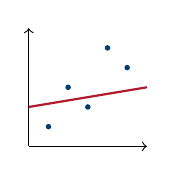
\begin{tikzpicture}[scale=0.5]
                    \draw[->] (0,0) -- (3,0);
                    \draw[->] (0,0) -- (0,3);
                    \fill[uibblue] (0.5,0.5) circle (2pt);
                    \fill[uibblue] (1,1.5) circle (2pt);
                    \fill[uibblue] (1.5,1) circle (2pt);
                    \fill[uibblue] (2,2.5) circle (2pt);
                    \fill[uibblue] (2.5,2) circle (2pt);
                    \draw[uibred, thick] (0,1) -- (3,1.5);
                \end{tikzpicture}
            \end{center}
        \end{column}

        \begin{column}{0.32\textwidth}
            \textbf{Good fit:}
            \begin{itemize}
                \item Right complexity
                \item Balance
                \item Generalizes well
            \end{itemize}
            \begin{center}
                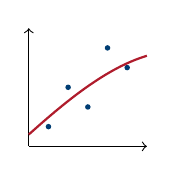
\begin{tikzpicture}[scale=0.5]
                    \draw[->] (0,0) -- (3,0);
                    \draw[->] (0,0) -- (0,3);
                    \fill[uibblue] (0.5,0.5) circle (2pt);
                    \fill[uibblue] (1,1.5) circle (2pt);
                    \fill[uibblue] (1.5,1) circle (2pt);
                    \fill[uibblue] (2,2.5) circle (2pt);
                    \fill[uibblue] (2.5,2) circle (2pt);
                    \draw[uibred, thick] (0,0.3) .. controls (1,1.2) and (2,2) .. (3,2.3);
                \end{tikzpicture}
            \end{center}
        \end{column}

        \begin{column}{0.32\textwidth}
            \textbf{Overfitting:}
            \begin{itemize}
                \item Too complex model
                \item High variance
                \item Learns noise in data
            \end{itemize}
            \begin{center}
                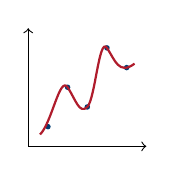
\begin{tikzpicture}[scale=0.5]
                    \draw[->] (0,0) -- (3,0);
                    \draw[->] (0,0) -- (0,3);
                    \fill[uibblue] (0.5,0.5) circle (2pt);
                    \fill[uibblue] (1,1.5) circle (2pt);
                    \fill[uibblue] (1.5,1) circle (2pt);
                    \fill[uibblue] (2,2.5) circle (2pt);
                    \fill[uibblue] (2.5,2) circle (2pt);
                    \draw[uibred, thick] (0.3,0.3) .. controls (0.6,0.6) and (0.8,1.8) .. (1,1.5) .. controls (1.2,1.2) and (1.3,0.8) .. (1.5,1) .. controls (1.7,1.2) and (1.8,2.8) .. (2,2.5) .. controls (2.2,2.2) and (2.3,1.8) .. (2.7,2.1);
                \end{tikzpicture}
            \end{center}
        \end{column}
    \end{columns}

    \vspace{3mm}
    \begin{block}{\footnotesize Signs of overfitting}
        \footnotesize Large difference between training and test \href{https://en.wikipedia.org/wiki/Evaluation_of_machine_learning_models}{performance}. \textbf{Performance} = measure of how well the model performs (e.g. accuracy, F1).
    \end{block}

\end{frame}

% ---------------------------------------------------------------------
% M06
% ---------------------------------------------------------------------
\begin{frame}{M06: \href{https://en.wikipedia.org/wiki/Bias\%E2\%80\%93variance_tradeoff}{Bias-Variance Trade-off}}

    \textbf{Total prediction error:}
    \[ \text{MSE} = \underbrace{\text{Bias}^2}_{\text{systematic error}} + \underbrace{\text{Variance}}_{\text{random error}} + \underbrace{\sigma^2}_{\text{irreducible}} \]

    \vspace{1mm}
    \begin{columns}
        \begin{column}{0.48\textwidth}
            \textbf{Bias (systematic error):}
            \begin{itemize}
                \item Error due to simplified model
                \item High bias $\rightarrow$ \textbf{underfitting}
                \item Model ``misses'' the pattern
            \end{itemize}

            \vspace{2mm}
            \textbf{Variance (random error):}
            \begin{itemize}
                \item Sensitive to small changes in data
                \item High variance $\rightarrow$ \textbf{overfitting}
                \item Model ``memorizes'' noise
            \end{itemize}
        \end{column}

        \begin{column}{0.48\textwidth}
            \begin{center}
                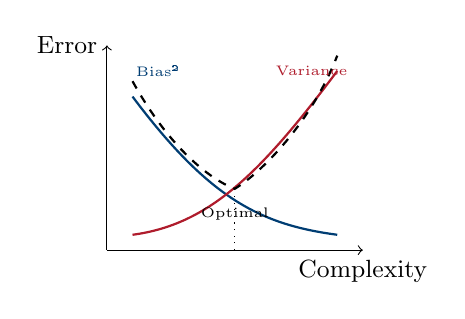
\begin{tikzpicture}[scale=0.65]
                    \draw[->] (0,0) -- (5,0) node[below] {\small Complexity};
                    \draw[->] (0,0) -- (0,4) node[left] {\small Error};

                    \draw[uibblue, thick] (0.5,3) .. controls (2,1) and (3,0.5) .. (4.5,0.3);
                    \draw[uibred, thick] (0.5,0.3) .. controls (2,0.5) and (3,1.5) .. (4.5,3.5);
                    \draw[black, thick, dashed] (0.5,3.3) .. controls (1.5,1.5) and (2.5,1.2) .. (2.5,1.2) .. controls (3,1.5) and (4,2.5) .. (4.5,3.8);

                    \node[uibblue] at (1, 3.5) {\tiny Bias²};
                    \node[uibred] at (4, 3.5) {\tiny Variance};
                    \node at (2.5, 0.7) {\tiny Optimal};

                    \draw[dotted] (2.5, 0) -- (2.5, 1.2);
                \end{tikzpicture}
            \end{center}
        \end{column}
    \end{columns}

    \begin{block}{\scriptsize The goal}
        \scriptsize Find the balance that minimizes \textbf{total error} on new data. $\sigma^2$ = noise in data (cannot be reduced).
    \end{block}

\end{frame}

% =====================================================================
\section{Validation and Model Types}
% =====================================================================

% ---------------------------------------------------------------------
% M07
% ---------------------------------------------------------------------
\begin{frame}{M07: \href{https://en.wikipedia.org/wiki/Cross-validation_(statistics)\#k-fold_cross-validation}{K-fold cross-validation}}
    
    \textbf{Problem:} A single train/test split can give random results
    
    \vspace{3mm}
    
    \textbf{Solution: K-fold Cross-Validation}
    \begin{enumerate}
        \item Split data into $k$ equal parts (``folds'')
        \item For each fold: use it as test, rest as training
        \item Average of all $k$ evaluations
    \end{enumerate}
    
    \vspace{3mm}
    
    \begin{center}
        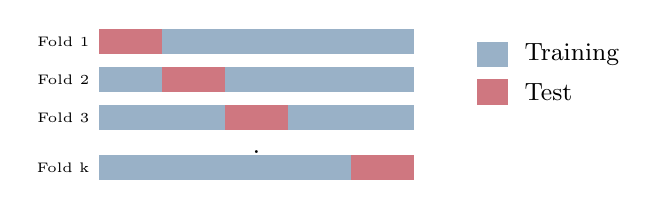
\begin{tikzpicture}[scale=0.8]
            % Fold 1
            \fill[uibred!60] (0,2) rectangle (1,2.4);
            \fill[uibblue!40] (1,2) rectangle (5,2.4);
            \node[left] at (0, 2.2) {\tiny Fold 1};
            
            % Fold 2
            \fill[uibblue!40] (0,1.4) rectangle (1,1.8);
            \fill[uibred!60] (1,1.4) rectangle (2,1.8);
            \fill[uibblue!40] (2,1.4) rectangle (5,1.8);
            \node[left] at (0, 1.6) {\tiny Fold 2};
            
            % Fold 3
            \fill[uibblue!40] (0,0.8) rectangle (2,1.2);
            \fill[uibred!60] (2,0.8) rectangle (3,1.2);
            \fill[uibblue!40] (3,0.8) rectangle (5,1.2);
            \node[left] at (0, 1) {\tiny Fold 3};
            
            % etc
            \node at (2.5, 0.4) {$\vdots$};
            
            \fill[uibblue!40] (0,0) rectangle (4,0.4);
            \fill[uibred!60] (4,0) rectangle (5,0.4);
            \node[left] at (0, 0.2) {\tiny Fold k};
            
            % Legend
            \fill[uibblue!40] (6, 1.8) rectangle (6.5, 2.2);
            \node[right] at (6.6, 2) {\small Training};
            \fill[uibred!60] (6, 1.2) rectangle (6.5, 1.6);
            \node[right] at (6.6, 1.4) {\small Test};
        \end{tikzpicture}
    \end{center}
    
    \vspace{3mm}
    
    \textbf{Advantages:} More robust estimate, uses all data for both training and testing
    
\end{frame}

% ---------------------------------------------------------------------
% M08
% ---------------------------------------------------------------------
\begin{frame}{M08: \href{https://en.wikipedia.org/wiki/Baseline_(machine_learning)}{Baseline model}}

    \begin{block}{\footnotesize What is a baseline?}
        \footnotesize A \textbf{simple reference model} that our ML model must beat to be useful.
    \end{block}

    \vspace{2mm}
    \textbf{Examples of baselines:}

    \begin{itemize}
        \item \textbf{Classification:} Always predict the majority class
        \begin{itemize}
            \item Dataset with 90\% healthy, 10\% sick $\rightarrow$ baseline accuracy = 90\%
        \end{itemize}
        \item \textbf{Regression:} Always predict the mean value
        \item \textbf{Time series:} Use previous value as prediction
    \end{itemize}

    \vspace{2mm}
    \begin{alertblock}{\footnotesize Why important?}
        \footnotesize
        90\% accuracy sounds impressive, but not if baseline is 90\%! Shows whether ML adds \textbf{actual value}. Reveals imbalanced datasets.
    \end{alertblock}

\end{frame}

% ---------------------------------------------------------------------
% M09
% ---------------------------------------------------------------------
\begin{frame}{M09: \href{https://en.wikipedia.org/wiki/Statistical_classification}{Classification} vs. \href{https://en.wikipedia.org/wiki/Regression_analysis}{Regression}}

    \begin{columns}
        \begin{column}{0.48\textwidth}
            \textbf{\faThLarge\ Classification:}
            \begin{itemize}
                \item Predicts \textbf{categories/classes}
                \item Discrete outcomes
                \item Examples:
                \begin{itemize}
                    \item Sick / Healthy
                    \item Cancer type A / B / C
                \end{itemize}
            \end{itemize}

            \vspace{2mm}
            \textbf{Evaluation metrics:}
            \footnotesize
            \begin{itemize}
                \item \href{https://en.wikipedia.org/wiki/Accuracy_and_precision\#In_classification}{Accuracy}, \href{https://en.wikipedia.org/wiki/Precision_and_recall\#Precision}{Precision}, \href{https://en.wikipedia.org/wiki/Precision_and_recall\#Recall}{Recall}
                \item \href{https://en.wikipedia.org/wiki/F-score}{F1-score}, \href{https://en.wikipedia.org/wiki/Receiver_operating_characteristic}{AUC-ROC}
            \end{itemize}
        \end{column}

        \begin{column}{0.48\textwidth}
            \textbf{\faChartLine\ Regression:}
            \begin{itemize}
                \item Predicts \textbf{continuous values}
                \item Numerical outcomes
                \item Examples:
                \begin{itemize}
                    \item Blood pressure
                    \item Drug dosage
                \end{itemize}
            \end{itemize}

            \vspace{2mm}
            \textbf{Evaluation metrics:}
            \footnotesize
            \begin{itemize}
                \item \href{https://en.wikipedia.org/wiki/Mean_squared_error}{MSE}, \href{https://en.wikipedia.org/wiki/Root-mean-square_deviation}{RMSE}, \href{https://en.wikipedia.org/wiki/Mean_absolute_error}{MAE}
                \item \href{https://en.wikipedia.org/wiki/Coefficient_of_determination}{R²} (explained variance)
            \end{itemize}
        \end{column}
    \end{columns}

\end{frame}

% ---------------------------------------------------------------------
% M10
% ---------------------------------------------------------------------
\begin{frame}{M10: Simple ML models}

    \begin{columns}
        \begin{column}{0.32\textwidth}
            \textbf{\href{https://en.wikipedia.org/wiki/Decision_tree_learning}{Decision tree}:}
            \begin{itemize}
                \item Series of yes/no questions
                \item Easy to interpret
                \item Can overfit
            \end{itemize}
            \begin{center}
                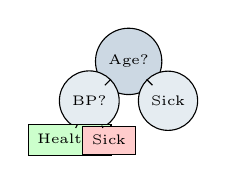
\begin{tikzpicture}[scale=0.5, every node/.style={font=\tiny}]
                    \node[draw, circle, fill=uibblue!20] (root) at (1.5,2) {Age?};
                    \node[draw, circle, fill=uibblue!10] (l) at (0.5,1) {BP?};
                    \node[draw, circle, fill=uibblue!10] (r) at (2.5,1) {Sick};
                    \node[draw, rectangle, fill=green!20] (ll) at (0,0) {Healthy};
                    \node[draw, rectangle, fill=red!20] (lr) at (1,0) {Sick};
                    \draw (root) -- (l);
                    \draw (root) -- (r);
                    \draw (l) -- (ll);
                    \draw (l) -- (lr);
                \end{tikzpicture}
            \end{center}
        \end{column}
        
        \begin{column}{0.32\textwidth}
            \textbf{\href{https://en.wikipedia.org/wiki/K-nearest_neighbors_algorithm}{k-Nearest Neighbors}:}
            \begin{itemize}
                \item Find $k$ most similar examples
                \item Majority voting
                \item Simple, but slow
            \end{itemize}
            \begin{center}
                
\begin{tikzpicture}[scale=0.5]
                    \fill[uibblue] (0.5,0.5) circle (3pt);
                    \fill[uibblue] (0.8,1) circle (3pt);
                    \fill[uibblue] (1,0.7) circle (3pt);
                    \fill[uibred] (2,2) circle (3pt);
                    \fill[uibred] (2.3,1.8) circle (3pt);
                    \fill[uibred] (1.8,2.2) circle (3pt);
                    \node[draw, star, fill=green!50, scale=0.5] at (1.5,1.3) {};
                    \draw[dashed] (1.5,1.3) circle (0.6);
                \end{tikzpicture}
            \end{center}
        \end{column}
        
        \begin{column}{0.32\textwidth}
            \textbf{\href{https://en.wikipedia.org/wiki/Logistic_regression}{Logistic regression}:}
            \begin{itemize}
                \item Linear boundary
                \item Gives probabilities
                \item Fast and interpretable
            \end{itemize}
            \begin{center}
                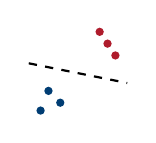
\begin{tikzpicture}[scale=0.5]
                    \fill[uibblue] (0.3,0.3) circle (3pt);
                    \fill[uibblue] (0.5,0.8) circle (3pt);
                    \fill[uibblue] (0.8,0.5) circle (3pt);
                    \fill[uibred] (2,2) circle (3pt);
                    \fill[uibred] (2.2,1.7) circle (3pt);
                    \fill[uibred] (1.8,2.3) circle (3pt);
                    \draw[thick, dashed] (0,1.5) -- (2.5,1);
                \end{tikzpicture}
            \end{center}
        \end{column}
    \end{columns}
    
    \vspace{5mm}
    
    \begin{block}{Tip}
        Always start with simple models before trying complex ones!
    \end{block}
    
\end{frame}

% ---------------------------------------------------------------------
% Summary
% ---------------------------------------------------------------------
\begin{frame}{Summary: M01--M10}
    \vspace{-2mm}
    \begin{columns}
        \begin{column}{0.32\textwidth}
            \textbf{\footnotesize Key concepts:}
            \scriptsize
            \begin{itemize}\setlength{\itemsep}{0pt}
                \item ML learns from data
                \item Supervised / Unsupervised / Semi-supervised
                \item Features (X), Labels (y)
                \item Training / test / validation
                \item Over-/underfitting
            \end{itemize}
        \end{column}
        \begin{column}{0.32\textwidth}
            \textbf{\footnotesize Best practices:}
            \scriptsize
            \begin{itemize}\setlength{\itemsep}{0pt}
                \item Cross-validation
                \item Compare with baseline
                \item Classification $\neq$ Regression
                \item Start simple
                \item Bias-variance balance
            \end{itemize}
        \end{column}
        \begin{column}{0.34\textwidth}
            \textbf{\footnotesize Future: ML + GenAI}
            \scriptsize
            \begin{itemize}\setlength{\itemsep}{0pt}
                \item LLM agents for data analysis
                \item Multimodal models (text+image)
                \item RAG + clinical guidelines
                \item Automated ML pipeline
                \item Human-in-the-loop AI
            \end{itemize}
        \end{column}
    \end{columns}

    \vspace{0mm}
    \begin{block}{\scriptsize Medical relevance -- ML applications in health, medicine and biotechnology}
        \scriptsize
        \textbf{Diagnostics:} Image diagnostics (radiology, pathology, ophthalmology, dermatology), biomarker detection, ECG/EEG analysis.\\
        \textbf{Prognosis:} Overall survival (OS), progression-free survival (PFS), readmission, mortality risk, disease progression.\\
        \textbf{Therapy:} Treatment selection, dose optimization, treatment response, radiation planning, surgical navigation.\\
        \textbf{Drug development:} Drugability, target identification, ADMET prediction, virtual screening, de novo molecule design.\\
        \textbf{Healthcare system:} Resource allocation, capacity planning, triage, waitlist optimization, outbreak detection.\\
        \textbf{Genomics/biotech:} Variant classification, gene expression, protein structure (AlphaFold), single-cell, CRISPR off-target.\\
        \textbf{Psychiatry/neurology:} Sentiment analysis, speech markers, neurodegeneration, seizure prediction.\\
        \textbf{Public health:} Epidemiological modeling, vaccine strategy, social determinants, health economics (QALY/DALY).
    \end{block}
    
    \vspace{-1mm}
    \begin{center}
    \tiny\textbf{Human-in-the-loop:} Patient image $\rightarrow$ \fbox{ML: ``possible malignant'' (87\%)} $\rightarrow$ Radiologist evaluates $\rightarrow$ Confirms/rejects $\rightarrow$ Feedback $\rightarrow$ Model improves
    \end{center}

\end{frame}

\end{document}
